\documentclass[tikz]{standalone}
\usetikzlibrary{patterns}
\usetikzlibrary{shapes,arrows}
\usetikzlibrary{decorations.pathreplacing, positioning}
\definecolor{greengreen}{rgb}{0.0, 0.42, 0.24}
\definecolor{calpolypomonagreen}{rgb}{0.12, 0.3, 0.17}
\definecolor{forestgreen}{rgb}{0.13, 0.55, 0.13}

\begin{document}
\noindent
  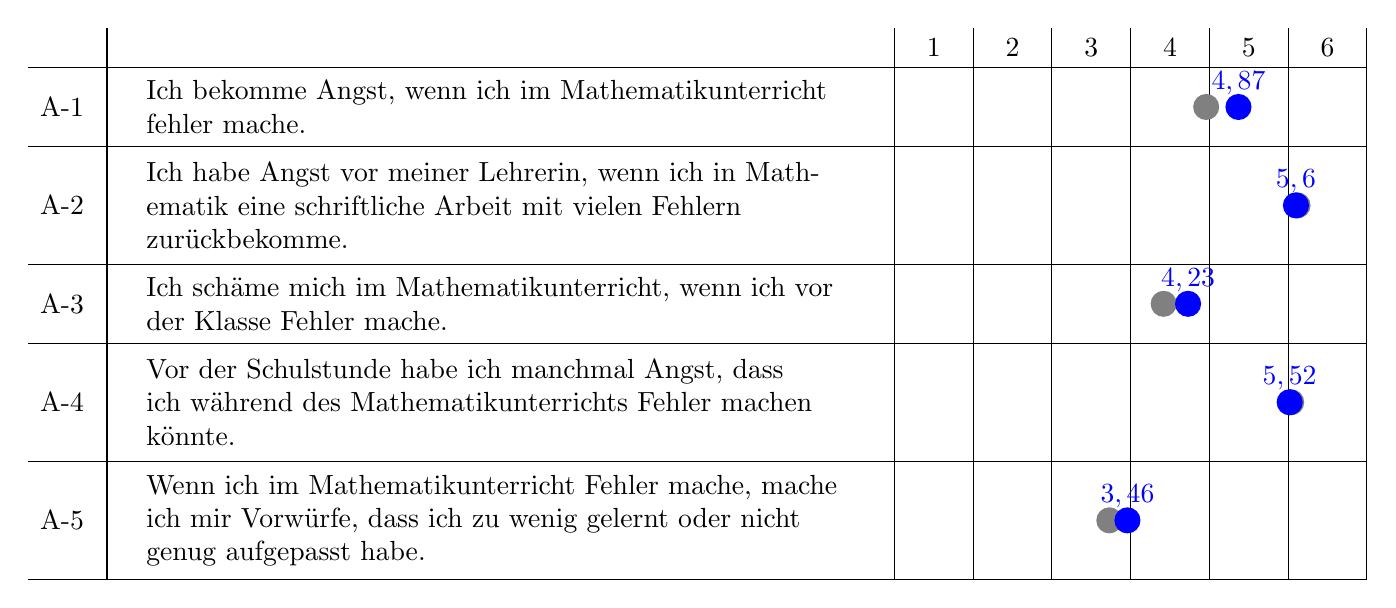
\begin{tikzpicture}

    \foreach \y in {0,1,2.5,3.5,5,6.5}
        \draw (-1, 0 - \y) -- (16, 0 - \y);
    \foreach \x in {0,10,11,12,13,14,15,16}
        \draw (0 + \x, 0.5) -- (0 + \x, - 6.5);
    
    \node at (10.5, 0.25) {$1$};
    \node at (11.5, 0.25) {$2$};
    \node at (12.5, 0.25) {$3$};
    \node at (13.5, 0.25) {$4$};
    \node at (14.5, 0.25) {$5$};
    \node at (15.5, 0.25) {$6$};

    \node[thick, align=left, text width=1cm] at (-0.35, -0.5) {A-1};
    \node[thick, align=left, text width=9cm] at (5, -0.5) {Ich bekomme Angst, wenn ich im Mathematikunterricht fehler mache.};
    \node[thick, circle, fill=gray, minimum width=0.25] (1) at (9.5 + 4.46, -0.5) {};
    \node[thick, blue] at (9.5 + 4.87, -0.2) {$4,87$};
    \node[thick, circle, fill=blue, minimum width=0.25] (1) at (9.5 + 4.87, -0.5) {};


    \node[thick, align=left, text width=1cm] at (-0.35, -1.75) {A-2};
    \node[thick, align=left, text width=9cm] at (5, -1.75) {Ich habe Angst vor meiner Lehrerin, wenn ich in Mathematik eine schriftliche Arbeit mit vielen Fehlern zurückbekomme.};
    \node[thick, blue] at (9.5 + 5.6, -1.45) {$5,6$};
    \node[thick, circle, fill=gray, minimum width=0.25] (2) at (9.5 + 5.62, -1.75) {};
    \node[thick, circle, fill=blue, minimum width=0.25] (1) at (9.5 + 5.6, -1.75) {};


    \node[thick, align=left, text width=1cm] at (-0.35, -3) {A-3};
    \node[thick, align=left, text width=9cm] at (5, -3) {Ich schäme mich im Mathematikunterricht, wenn ich vor der Klasse Fehler mache.};
    \node[thick, blue] at (9.5 + 4.23, -2.7) {$4,23$};
    \node[thick, circle, fill=gray, minimum width=0.25] (3) at (9.5 + 3.92, -3) {};
    \node[thick, circle, fill=blue, minimum width=0.25] (1) at (9.5 + 4.23, -3) {};


    \node[thick, align=left, text width=1cm] at (-0.35, -4.25) {A-4};
    \node[thick, align=left, text width=9cm] at (5, -4.25) {Vor der Schulstunde habe ich manchmal Angst, dass ich während des Mathematikunterrichts Fehler machen könnte.};
    \node[thick, blue] at (9.5 + 5.52, -3.95) {$5,52$};
    \node[thick, circle, fill=gray, minimum width=0.25] (4) at (9.5 + 5.54, -4.25) {};
    \node[thick, circle, fill=blue, minimum width=0.25] (1) at (9.5 + 5.52, -4.25) {};


    \node[thick, align=left, text width=1cm] at (-0.35, -5.75) {A-5};
    \node[thick, align=left, text width=9cm] at (5, -5.75) {Wenn ich im Mathematikunterricht Fehler mache, mache ich mir Vorwürfe, dass ich zu wenig gelernt oder nicht genug aufgepasst habe.};
    \node[thick, blue] at (9.5 + 3.46, -5.45) {$3,46$};
    \node[thick, circle, fill=gray, minimum width=0.25] (5) at (9.5 + 3.23, -5.75) {};
    \node[thick, circle, fill=blue, minimum width=0.25] (1) at (9.5 + 3.46, -5.75) {};
    
    

    

    %\draw[color=blue, thick] (1) to (2) to (3) to (4) to (5);

  \end{tikzpicture}%
\end{document}
